\documentclass{article}
\usepackage{graphicx}
\usepackage{amsmath}
\usepackage{amssymb}
\usepackage{listings}
\usepackage[margin=1in]{geometry}
\usepackage{xcolor}
\usepackage{tikz}
\usetikzlibrary{shapes, arrows, positioning, calc, shapes.geometric}
\usepackage{pgfplots}
\pgfplotsset{compat=1.18}
\usepackage{tcolorbox}
\usepackage{multirow}

% Define colors for syntax highlighting
\definecolor{codegreen}{rgb}{0,0.6,0}
\definecolor{codegray}{rgb}{0.5,0.5,0.5}
\definecolor{codepurple}{rgb}{0.58,0,0.82}
\definecolor{backcolour}{rgb}{0.95,0.95,0.92}

% Python style for highlighting
\lstdefinestyle{pythonstyle}{
    backgroundcolor=\color{backcolour},   
    commentstyle=\color{codegreen},
    keywordstyle=\color{magenta},
    numberstyle=\tiny\color{codegray},
    stringstyle=\color{codepurple},
    basicstyle=\ttfamily\footnotesize,
    breakatwhitespace=false,         
    breaklines=true,                 
    captionpos=b,                    
    keepspaces=true,                 
    numbers=left,                    
    numbersep=5pt,                  
    showspaces=false,                
    showstringspaces=false,
    showtabs=false,                  
    tabsize=2
}
\lstset{style=pythonstyle}

\title{Lecture: Efficient Training \& Inference for RNNs}
\author{Deep Learning Class}
\date{\today}

\begin{document}
\maketitle

\section{Introduction}

In our previous lectures, we introduced the fundamental architectures of recurrent neural networks: vanilla RNNs, LSTMs, and GRUs. We saw how these models can process sequential data and maintain hidden states to capture temporal dependencies.

However, training and deploying these models efficiently in practice requires careful consideration of several key techniques. This creates what practitioners call the \textbf{``triple constraint''}: the need to constantly balance three competing objectives:

\begin{enumerate}
\item \textbf{Model performance} (e.g., translation accuracy, BLEU score)
\item \textbf{Training time} (development velocity and computational budget)
\item \textbf{Inference latency} (critical for user-facing applications)
\end{enumerate}

\begin{tcolorbox}[colback=yellow!5!white, colframe=orange!50!black, title=The Efficiency Imperative]
A model that is theoretically powerful but practically inefficient may be of limited value. In both research and industry, efficiency is not optional—it directly impacts:
\begin{itemize}
\item Research iteration speed (more experiments per day)
\item Infrastructure costs (GPU hours, cloud compute)
\item User experience (latency in production systems)
\item Environmental impact (energy consumption)
\end{itemize}
\end{tcolorbox}

Today, we will explore methods that make RNN training faster and inference more effective. These concepts lay critical groundwork for understanding modern architectures like Transformers, where many of these same principles apply.

\textbf{Roadmap:}
\begin{itemize}
\item \textbf{Efficient Training Techniques}: Teacher forcing, exposure bias, and masking
\item \textbf{Efficient Inference Strategies}: Batched inference, greedy search, and beam search
\end{itemize}

\section{Teacher Forcing: Accelerating Training}

\subsection{Motivation}

Consider training a sequence-to-sequence model (e.g., machine translation). At each timestep $t'$, the decoder must predict the next token $y_{t'}$ given:
\begin{itemize}
\item The encoder context vector $\mathbf{c}$
\item The previous outputs $y_1, \ldots, y_{t'-1}$
\end{itemize}

\textbf{The naive approach} (``free-running'' decoder) would be to feed the model's own predictions back as inputs during training. This creates a vicious cycle:

\begin{center}
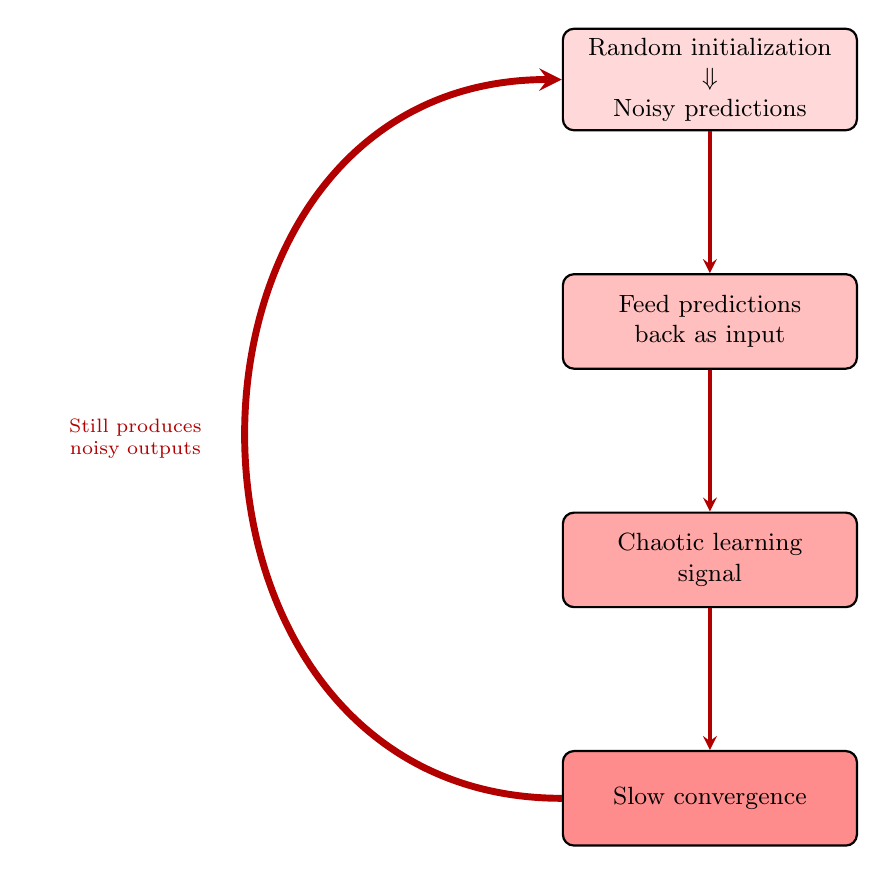
\begin{tikzpicture}[
    node distance=1.8cm,
    box/.style={rectangle, draw, thick, fill=red!20, rounded corners, text width=3.5cm, align=center, minimum height=1.2cm, font=\small},
    arrow/.style={->, >=stealth, very thick, red!70!black}
]

\node[box, fill=red!15] (init) {Random initialization\\ $\Downarrow$ \\ Noisy predictions};
\node[box, fill=red!25, below=of init] (feedback) {Feed predictions\\ back as input};
\node[box, fill=red!35, below=of feedback] (chaos) {Chaotic learning\\ signal};
\node[box, fill=red!45, below=of chaos] (slow) {Slow convergence};

\draw[arrow] (init) -- (feedback);
\draw[arrow] (feedback) -- (chaos);
\draw[arrow] (chaos) -- (slow);
\draw[arrow, line width=2.5pt] (slow.west) to[out=180, in=180, looseness=1.5] node[left, text width=2.5cm, align=center, font=\scriptsize] {Still produces\\ noisy outputs} (init.west);

\end{tikzpicture}
\end{center}

\textbf{Two critical problems}:
\begin{enumerate}
\item \textbf{Sequential dependency}: We must wait for prediction at $t'-1$ before computing timestep $t'$
\item \textbf{Error accumulation}: Early mistakes compound throughout the sequence—the model learns to translate \textit{and} recover from cascading errors simultaneously
\end{enumerate}

\begin{tcolorbox}[colback=red!5!white, colframe=red!50!black, title=Empirical Impact of Free-Running Training]
In experiments on English-German translation (Multi30k dataset):
\begin{itemize}
\item \textbf{Average training time per epoch}: 18.5 minutes
\item \textbf{Epochs to reach validation loss of 3.5}: 8 epochs
\item \textbf{Final BLEU score}: 19.8

\end{itemize}
The optimization landscape becomes extremely difficult to navigate, resulting in painfully slow convergence.
\end{tcolorbox}

\subsection{The Teacher Forcing Strategy}

\textbf{Core idea}: During training, use the ground-truth token $y_{t'-1}$ as input to the decoder at timestep $t'$, rather than the model's prediction.

\begin{tcolorbox}[colback=blue!5!white, colframe=blue!50!black, title=Teacher Forcing Definition]
In \textbf{teacher forcing}, the decoder receives the actual target sequence as input during training:
\[
\text{Decoder input at } t': \quad y_{t'-1}^{\text{ground-truth}} \quad \text{instead of} \quad \hat{y}_{t'-1}^{\text{predicted}}
\]
The special $\langle \text{bos} \rangle$ (beginning-of-sequence) token starts the process, and the original target sequence (excluding the final token) is concatenated as decoder input.
\end{tcolorbox}

\subsection{Architecture Comparison}

Let's visualize how teacher forcing changes the computational graph:

\begin{center}
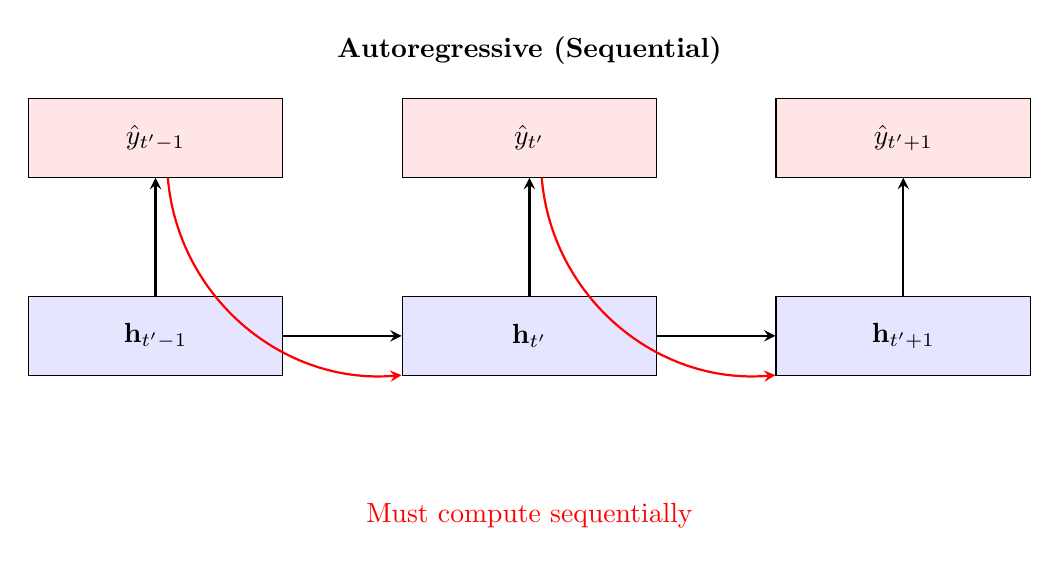
\begin{tikzpicture}[
    node distance=1.5cm,
    block/.style={rectangle, draw, fill=blue!10, text width=3cm, text centered, minimum height=1cm},
    arrow/.style={->, >=stealth, thick}
]

% Standard Autoregressive
\node[block] (h1) {$\mathbf{h}_{t'-1}$};
\node[block, right=of h1] (h2) {$\mathbf{h}_{t'}$};
\node[block, right=of h2] (h3) {$\mathbf{h}_{t'+1}$};

\node[block, above=of h1, fill=red!10] (o1) {$\hat{y}_{t'-1}$};
\node[block, above=of h2, fill=red!10] (o2) {$\hat{y}_{t'}$};
\node[block, above=of h3, fill=red!10] (o3) {$\hat{y}_{t'+1}$};

\draw[arrow] (h1) -- (o1);
\draw[arrow] (h2) -- (o2);
\draw[arrow] (h3) -- (o3);
\draw[arrow] (h1) -- (h2);
\draw[arrow] (h2) -- (h3);
\draw[arrow, red, thick] (o1) to[bend right=45] (h2);
\draw[arrow, red, thick] (o2) to[bend right=45] (h3);

\node[above=0.3cm of o2] {\textbf{Autoregressive (Sequential)}};
\node[below=1.5cm of h2, text=red] {Must compute sequentially};

\end{tikzpicture}
\end{center}

\begin{center}
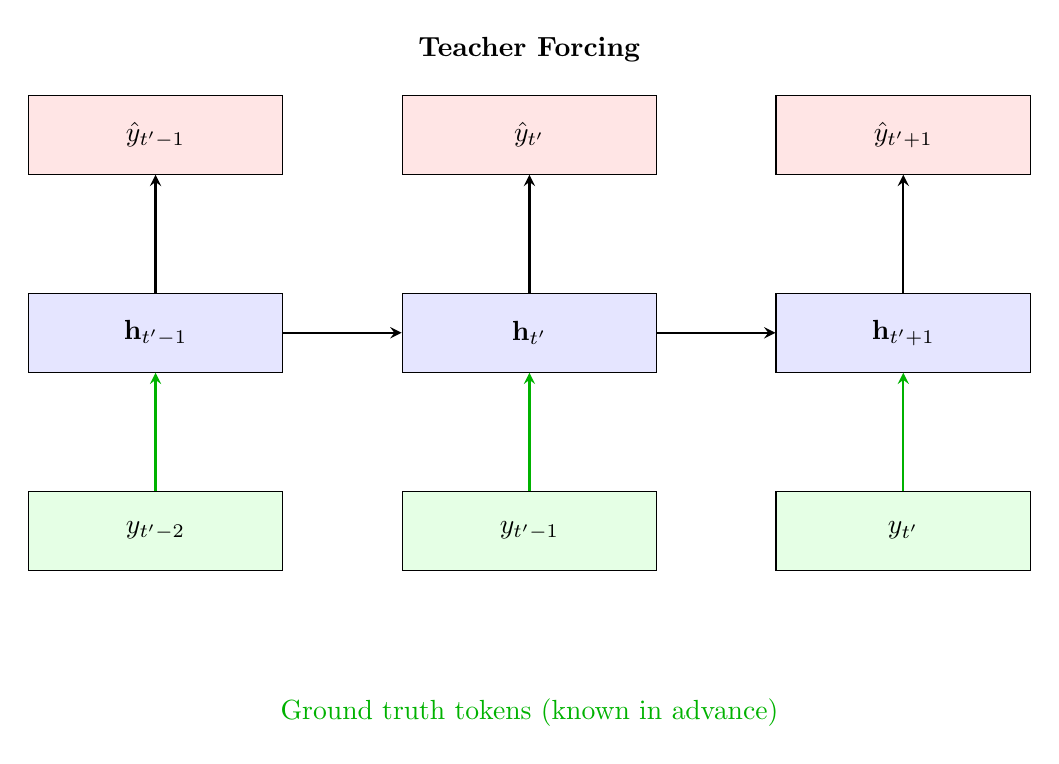
\begin{tikzpicture}[
    node distance=1.5cm,
    block/.style={rectangle, draw, fill=blue!10, text width=3cm, text centered, minimum height=1cm},
    arrow/.style={->, >=stealth, thick}
]

% Teacher Forcing
\node[block] (h1) {$\mathbf{h}_{t'-1}$};
\node[block, right=of h1] (h2) {$\mathbf{h}_{t'}$};
\node[block, right=of h2] (h3) {$\mathbf{h}_{t'+1}$};

\node[block, above=of h1, fill=red!10] (o1) {$\hat{y}_{t'-1}$};
\node[block, above=of h2, fill=red!10] (o2) {$\hat{y}_{t'}$};
\node[block, above=of h3, fill=red!10] (o3) {$\hat{y}_{t'+1}$};

\node[block, below=of h1, fill=green!10] (y1) {$y_{t'-2}$};
\node[block, below=of h2, fill=green!10] (y2) {$y_{t'-1}$};
\node[block, below=of h3, fill=green!10] (y3) {$y_{t'}$};

\draw[arrow] (h1) -- (o1);
\draw[arrow] (h2) -- (o2);
\draw[arrow] (h3) -- (o3);
\draw[arrow] (h1) -- (h2);
\draw[arrow] (h2) -- (h3);
\draw[arrow, green!70!black, thick] (y1) -- (h1);
\draw[arrow, green!70!black, thick] (y2) -- (h2);
\draw[arrow, green!70!black, thick] (y3) -- (h3);

\node[above=0.3cm of o2] {\textbf{Teacher Forcing}};
\node[below=1.5cm of y2, text=green!70!black] {Ground truth tokens (known in advance)};

\end{tikzpicture}
\end{center}

\subsection{Benefits of Teacher Forcing}

\begin{enumerate}
\item \textbf{Faster convergence}: Model always trains on correct context
\item \textbf{Stable gradients}: No error accumulation during training
\item \textbf{Parallelization potential}: With certain architectures (no hidden state recurrence), timesteps become independent
\item \textbf{Simpler optimization}: Loss computation is straightforward
\end{enumerate}

\begin{tcolorbox}[colback=green!5!white, colframe=green!50!black, title=Empirical Impact: Teacher Forcing]
\textbf{Experiment}: Train identical models on English-German translation, varying only the training strategy.

\vspace{0.3cm}
\begin{center}
\begin{tabular}{|l|c|c|}
\hline
\textbf{Metric} & \textbf{Free-Running} & \textbf{Teacher Forcing} \\
\hline
Avg. time per epoch & 18.5 min & 2.1 min \\
\hline
Epochs to loss $<$ 3.5 & 8 & 2 \\
\hline
\textbf{Speedup} & \textbf{1×} & \textbf{8.8×} \\
\hline
\end{tabular}
\end{center}

\vspace{0.3cm}
\textbf{The causal chain}:
\begin{enumerate}
\item Ground-truth inputs $\rightarrow$ clean gradient at each step
\item Clean gradients $\rightarrow$ confident optimization steps  
\item Confident steps $\rightarrow$ faster convergence
\item Result: \textbf{88.6\% reduction in training time per epoch}
\end{enumerate}

This is not a marginal improvement—it transforms experimentation speed and computational costs.
\end{tcolorbox}

\subsection{The Exposure Bias Problem}

\begin{tcolorbox}[colback=red!5!white, colframe=red!50!black, title=Exposure Bias]
\textbf{The mismatch}: During training, the decoder sees perfect ground-truth inputs. During inference, it must condition on its own imperfect predictions. This discrepancy is called \textbf{exposure bias}.
\end{tcolorbox}

\textbf{Consequences}:
\begin{itemize}
\item Model never learns to recover from its own mistakes
\item Errors accumulate at inference time
\item Performance degrades on longer sequences
\end{itemize}

\begin{center}
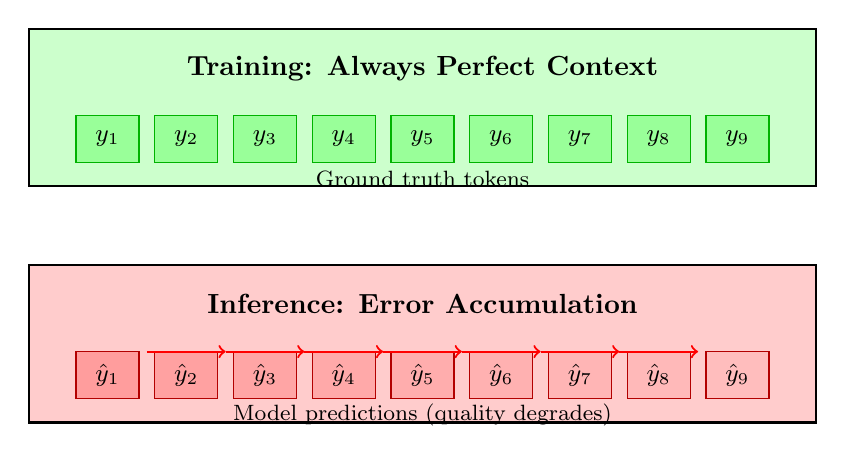
\begin{tikzpicture}
% Training scenario
\draw[thick, fill=green!20] (0,0) rectangle (10,2);
\node at (5, 1.5) {\textbf{Training: Always Perfect Context}};
\foreach \x in {1,...,9} {
    \draw[green!70!black, fill=green!40] (\x*1-0.4, 0.3) rectangle (\x*1+0.4, 0.9);
    \node at (\x, 0.6) {\small $y_{\x}$};
}
\node at (5, 0.1) {\footnotesize Ground truth tokens};

% Inference scenario
\draw[thick, fill=red!20] (0,-3) rectangle (10,-1);
\node at (5, -1.5) {\textbf{Inference: Error Accumulation}};
\foreach \x in {1,...,9} {
    \pgfmathsetmacro{\opacity}{1-0.08*\x}
    \draw[red!70!black, fill=red!40, fill opacity=\opacity] (\x*1-0.4, -2.7) rectangle (\x*1+0.4, -2.1);
    \node at (\x, -2.4) {\small $\hat{y}_{\x}$};
}
\node at (5, -2.9) {\footnotesize Model predictions (quality degrades)};

% Arrows showing degradation
\foreach \x in {2,...,8} {
    \draw[->, thick, red] (\x-0.5, -2.1) -- (\x+0.5, -2.1);
}

\end{tikzpicture}
\end{center}

\subsection{Solution: Scheduled Sampling}

To mitigate exposure bias, we can use \textbf{scheduled sampling}: gradually transition from teacher forcing to using model predictions during training.

This approach was formalized by Bengio et al. (2015) in their paper ``Scheduled Sampling for Sequence Prediction with Recurrent Neural Networks'' and was successfully used in their winning entry to the MSCOCO 2015 image captioning challenge.

\subsubsection{The Core Algorithm}

At each timestep during training, flip a biased coin with probability $\epsilon_i$ (where $i$ is the training iteration):
\begin{itemize}
\item With probability $\epsilon_i$: use ground truth token $y_{t-1}$ (teacher forcing)
\item With probability $(1-\epsilon_i)$: use model prediction $\hat{y}_{t-1}$
\end{itemize}

\begin{tcolorbox}[colback=orange!5!white, colframe=orange!50!black, title=Important Design Choice]
\textbf{Flip per token, not per sequence!} Bengio et al. found that flipping once per sequence yielded ``much worse'' results, ``most probably because consecutive errors are amplified during the first rounds of training.''
\end{tcolorbox}

\begin{lstlisting}[language=Python, caption=Scheduled Sampling Implementation]
def scheduled_sampling(epoch, max_epochs, schedule='linear'):
    if schedule == 'linear':
        epsilon = max(eps_min, k - c * epoch)
    elif schedule == 'exponential':
        epsilon = k ** epoch
    elif schedule == 'inverse_sigmoid':
        epsilon = k / (k + exp(epoch / k))
    return epsilon

# During training
epsilon_i = scheduled_sampling(epoch, max_epochs)
for t in range(seq_len):
    if random() < epsilon_i:
        decoder_input = ground_truth[t-1]  # Teacher forcing
    else:
        # Sample from model or take argmax
        decoder_input = sample_from_model(output_dist)
    
    hidden, output = decoder(decoder_input, hidden)
\end{lstlisting}

\subsubsection{Decay Schedules}

Bengio et al. propose three curriculum schedules for $\epsilon_i$:

\textbf{1. Linear Decay}:
\[
\epsilon_i = \max(\epsilon_{\min}, k - c \cdot i)
\]
where $0 \leq \epsilon_{\min} < 1$ is the minimum teacher forcing ratio, and $k$, $c$ control offset and slope.

\textbf{2. Exponential Decay}:
\[
\epsilon_i = k^i \quad \text{where } k < 1
\]

\textbf{3. Inverse Sigmoid Decay}:
\[
\epsilon_i = \frac{k}{k + \exp(i/k)} \quad \text{where } k \geq 1
\]

\begin{center}
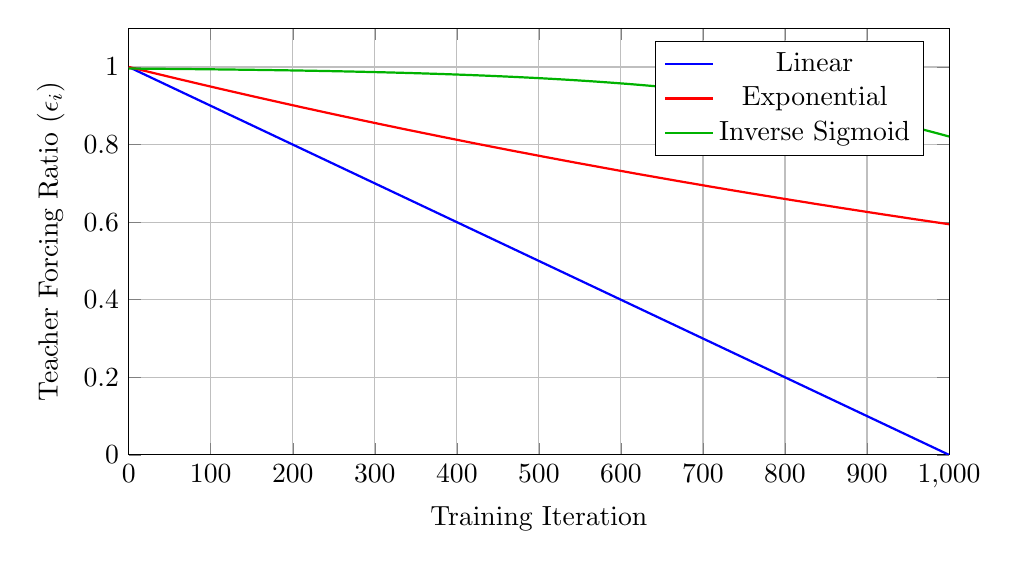
\begin{tikzpicture}
\begin{axis}[
    width=12cm, height=7cm,
    xlabel={Training Iteration},
    ylabel={Teacher Forcing Ratio ($\epsilon_i$)},
    xmin=0, xmax=1000,
    ymin=0, ymax=1.1,
    grid=major,
    legend pos=north east
]
\addplot[thick, blue, domain=0:1000, samples=100] {1 - x/1000};
\addplot[thick, red, domain=0:1000, samples=100] {0.9995^x};
\addplot[thick, green!70!black, domain=0:1000, samples=100] {250/(250 + exp(x/250))};
\legend{Linear, Exponential, Inverse Sigmoid}
\end{axis}
\end{tikzpicture}
\end{center}

The inverse sigmoid schedule is gentler at the beginning and end, which can help with training stability.

\subsubsection{Empirical Results}

Bengio et al. demonstrated consistent improvements across three diverse tasks:

\begin{center}
\begin{tabular}{|l|c|c|c|}
\hline
\textbf{Task} & \textbf{Baseline} & \textbf{Scheduled} & \textbf{Improvement} \\
\hline
Image Captioning (BLEU-4) & 28.8 & 30.6 & +6.2\% \\
Constituency Parsing (F1) & 86.54 & 88.08 & +1.8\% \\
Speech Recognition (FER) & 46.0 & 34.5 & -25\% (lower is better) \\
\hline
\end{tabular}
\end{center}

\vspace{0.3cm}

\textbf{Additional empirical evidence} from English-German translation experiments:

\begin{center}
\begin{tabular}{|l|c|c|}
\hline
\textbf{Training Method} & \textbf{Final BLEU Score} & \textbf{Improvement} \\
\hline
100\% Teacher Forcing & 25.4 & Baseline \\
Scheduled Sampling & 27.1 & +6.7\% \\
\hline
\end{tabular}
\end{center}

\textbf{Key insight}: While pure teacher forcing leads to \textit{faster initial convergence}, scheduled sampling produces a more \textit{robust model} that performs better under the uncertainty of real inference.

\begin{tcolorbox}[colback=red!5!white, colframe=red!50!black, title=Critical Warning]
\textbf{Never use 100\% sampling (``Always Sampling'')!}

When $\epsilon_i = 0$ from the start (always sampling from model), performance collapses:
\begin{itemize}
\item Image captioning: BLEU-4 drops to 11.2 (vs 28.8 baseline)
\item Parsing: Trees become invalid
\end{itemize}

\textbf{Why?} The model samples random tokens early in training $\rightarrow$ learns nothing meaningful $\rightarrow$ continues sampling garbage.

The curriculum is essential: start with easy task (teacher forcing), gradually increase difficulty.
\end{tcolorbox}

\section{Masking \& Handling Padded Sequences}

\subsection{The Padding Problem}

When processing batches of sequences, we encounter varying sequence lengths. To form a tensor, we must \textbf{pad} shorter sequences to match the longest one.

\textbf{Example batch}:
\begin{verbatim}
Sequence 1: [5, 2, 8, 9]         length = 4
Sequence 2: [3, 1]               length = 2
Sequence 3: [7, 4, 6]            length = 3
\end{verbatim}

After padding with special token $\langle \text{pad} \rangle = 0$:
\begin{verbatim}
Padded batch (max_len = 4):
[[5, 2, 8, 9],
 [3, 1, 0, 0],
 [7, 4, 6, 0]]
\end{verbatim}

\subsection{Why Masking Matters}

\textbf{Problem}: Padded positions should not contribute to:
\begin{itemize}
\item Loss computation
\item Gradient updates
\item Model predictions
\end{itemize}

\textbf{Solution}: Create a \textbf{mask} to identify real vs. padded tokens.

\subsection{Mask Construction}

A mask is a binary tensor with the same shape as the input:
\[
\text{mask}_{ij} = \begin{cases}
1 & \text{if position } j \text{ is a real token} \\
0 & \text{if position } j \text{ is padding}
\end{cases}
\]

For our example:
\begin{verbatim}
Mask:
[[1, 1, 1, 1],
 [1, 1, 0, 0],
 [1, 1, 1, 0]]
\end{verbatim}

\subsection{Masked Loss Computation}

The loss should only consider non-padded positions:
\[
\mathcal{L} = \frac{\sum_{i=1}^{B} \sum_{t=1}^{T} m_{it} \cdot \text{CE}(y_{it}, \hat{y}_{it})}{\sum_{i=1}^{B} \sum_{t=1}^{T} m_{it}}
\]

where:
\begin{itemize}
\item $B$ = batch size
\item $T$ = sequence length (padded)
\item $m_{it}$ = mask value at position $(i,t)$
\item $\text{CE}$ = cross-entropy loss
\end{itemize}

\begin{lstlisting}[language=Python, caption=Masked Loss in PyTorch]
def masked_loss(predictions, targets, mask):
    """
    predictions: [batch, seq_len, vocab_size]
    targets: [batch, seq_len]
    mask: [batch, seq_len]
    """
    # Compute loss for all positions
    loss = F.cross_entropy(
        predictions.view(-1, vocab_size),
        targets.view(-1),
        reduction='none'
    )
    
    # Apply mask and normalize
    loss = loss * mask.view(-1)
    return loss.sum() / mask.sum()
\end{lstlisting}

\subsection{Preview: Causal Masking in Transformers}

\begin{tcolorbox}[colback=yellow!5!white, colframe=orange!50!black, title=Looking Ahead]
RNNs have \textbf{inherent causal structure}: at time $t$, the hidden state $\mathbf{h}_t$ can only depend on $x_1, \ldots, x_t$ due to sequential processing.

In \textbf{Transformers}, which process all positions in parallel, we must explicitly enforce this causality using a \textbf{causal mask} (also called attention mask):
\[
\text{CausalMask}_{ij} = \begin{cases}
0 & \text{if } i < j \text{ (can attend)} \\
-\infty & \text{if } i \geq j \text{ (cannot attend)}
\end{cases}
\]

This prevents position $i$ from ``peeking'' at future positions $j > i$.
\end{tcolorbox}

\section{Batched Inference \& Sequence Bucketing}

\subsection{The Throughput Problem}

At inference time, we often process many sequences. Naive batching leads to massive waste:

\textbf{Concrete Example}: Batch of 4 sequences with lengths [12, 28, 9, 15]

\begin{itemize}
\item Naive padding: all padded to length 28
\item Total tokens processed: $4 \times 28 = 112$
\item Actual meaningful tokens: $12 + 28 + 9 + 15 = 64$
\item \textbf{Wasted computation: $\frac{48}{112} = 43\%$}
\end{itemize}

\begin{center}
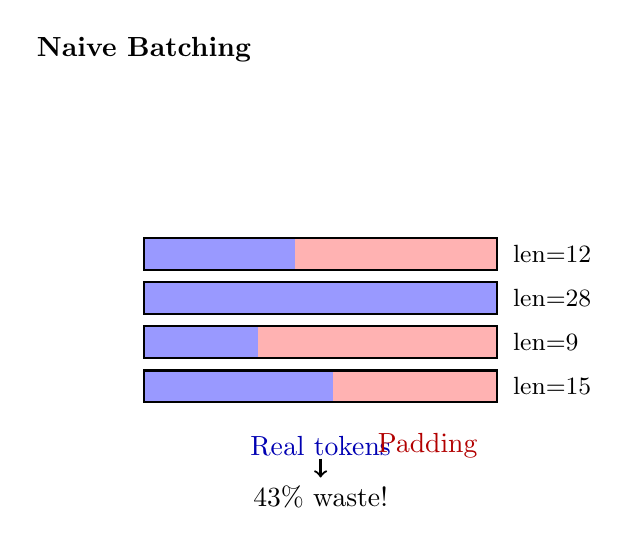
\begin{tikzpicture}[scale=0.8]
% Naive batch visualization
\node at (0, 3) {\textbf{Naive Batching}};

\foreach \y/\len in {0/12, 1/28, 2/9, 3/15} {
    % Actual tokens
    \fill[blue!40] (0, -\y*0.7) rectangle (\len*0.2, -\y*0.7-0.5);
    % Padding
    \fill[red!30] (\len*0.2, -\y*0.7) rectangle (5.6, -\y*0.7-0.5);
    \draw[thick] (0, -\y*0.7) rectangle (5.6, -\y*0.7-0.5);
    \node[right] at (5.7, -\y*0.7-0.25) {\small len=\len};
}

\node[blue!70!black] at (2.8, -3.3) {Real tokens};
\node[red!70!black] at (4.5, -3.3) {Padding};
\draw[->, thick] (2.8, -3.5) -- (2.8, -3.8);
\node at (2.8, -4.1) {43\% waste!};
\end{tikzpicture}
\end{center}

The RNN processes \textit{every} token, including padding. All matrix multiplications and activations on $\langle \text{pad} \rangle$ tokens consume GPU cycles but contribute \textit{nothing} to output.

\subsection{Sequence Bucketing Strategy}

\textbf{Solution}: Group sequences of similar lengths into ``buckets'', then process each bucket separately.

\textbf{Algorithm}:
\begin{enumerate}
\item Define length buckets: e.g., [0-10], [11-25], [26-50], [51-100], [100+]
\item Sort sequences by length
\item Group sequences into buckets
\item Pad within each bucket (minimal padding)
\item Process each bucket independently
\end{enumerate}

\begin{center}
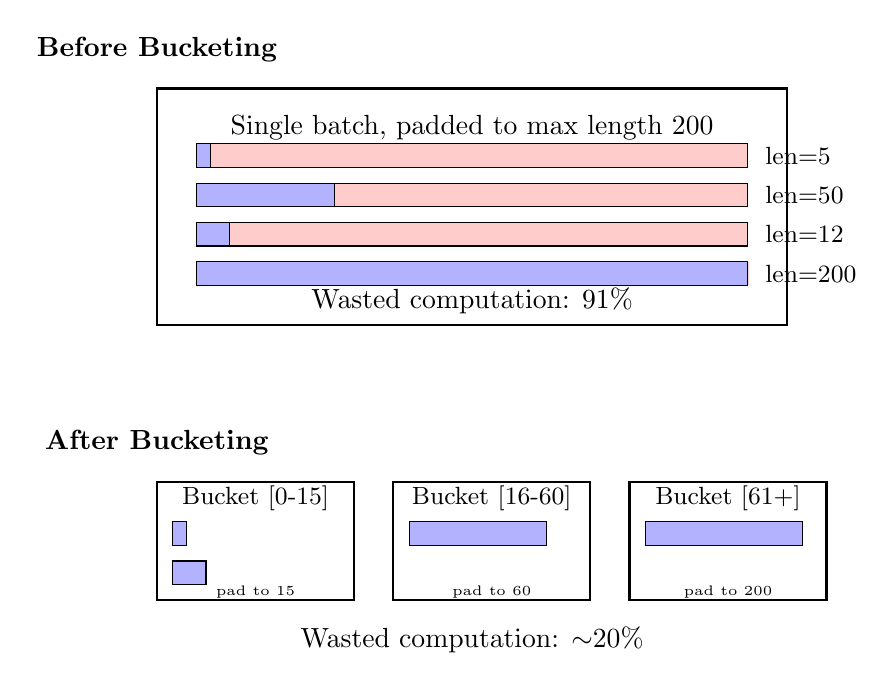
\begin{tikzpicture}
% Before bucketing
\node at (0, 4) {\textbf{Before Bucketing}};
\draw[thick] (0, 3.5) rectangle (8, 0.5);
\node at (4, 3) {Single batch, padded to max length 200};

\foreach \x/\len in {1/5, 2/50, 3/12, 4/200} {
    \draw[fill=blue!30] (0.5, 3-\x*0.5) rectangle (0.5+\len*0.035, 3-\x*0.5+0.3);
    \draw[fill=red!20] (0.5+\len*0.035, 3-\x*0.5) rectangle (7.5, 3-\x*0.5+0.3);
    \node[right] at (7.6, 3-\x*0.5+0.15) {\small len=\len};
}
\node at (4, 0.8) {Wasted computation: 91\%};

% After bucketing
\node at (0, -1) {\textbf{After Bucketing}};

% Bucket 1: short sequences
\draw[thick] (0, -1.5) rectangle (2.5, -3);
\node at (1.25, -1.7) {\small Bucket [0-15]};
\draw[fill=blue!30] (0.2, -2) rectangle (0.375, -2.3);
\draw[fill=blue!30] (0.2, -2.5) rectangle (0.62, -2.8);
\node at (1.25, -2.9) {\tiny pad to 15};

% Bucket 2: medium sequences
\draw[thick] (3, -1.5) rectangle (5.5, -3);
\node at (4.25, -1.7) {\small Bucket [16-60]};
\draw[fill=blue!30] (3.2, -2) rectangle (4.95, -2.3);
\node at (4.25, -2.9) {\tiny pad to 60};

% Bucket 3: long sequences
\draw[thick] (6, -1.5) rectangle (8.5, -3);
\node at (7.25, -1.7) {\small Bucket [61+]};
\draw[fill=blue!30] (6.2, -2) rectangle (8.2, -2.3);
\node at (7.25, -2.9) {\tiny pad to 200};

\node at (4, -3.5) {Wasted computation: $\sim$20\%};

\end{tikzpicture}
\end{center}

\subsection{Benefits}

\begin{itemize}
\item \textbf{Reduced waste}: Minimize padding overhead
\item \textbf{Better GPU utilization}: More actual work per operation
\item \textbf{Faster throughput}: Process more sequences per second
\item \textbf{Lower memory}: Smaller batch tensors
\end{itemize}

\begin{tcolorbox}[colback=green!5!white, colframe=green!50!black, title=Empirical Impact: Sequence Bucketing]
\textbf{Experiment}: Measure inference throughput on English-German translation test set.

\vspace{0.3cm}
\begin{center}
\begin{tabular}{|l|c|c|}
\hline
\textbf{Strategy} & \textbf{Throughput} & \textbf{Total Padding Tokens} \\
 & \textbf{(sent/sec)} & \textbf{(Test Set)} \\
\hline
Standard Padding & 18 & 54,832 \\
Sequence Bucketing & 31 & 9,915 \\
\hline
\textbf{Improvement} & \textbf{+72\%} & \textbf{-82\%} \\
\hline
\end{tabular}
\end{center}

\vspace{0.3cm}
\textbf{The causal chain}:
\begin{enumerate}
\item Computational work $\propto$ batch\_size $\times$ seq\_length
\item Bucketing ensures seq\_length $\approx$ average actual length
\item Reduces total FLOPs by 80\%
\item Result: \textbf{72\% increase in inference throughput}
\end{enumerate}

This is a ``free'' performance gain—no changes to model architecture, just smarter data organization.
\end{tcolorbox}

\begin{tcolorbox}[colback=green!5!white, colframe=green!50!black, title=Hardware-Aware Optimization]
Sequence bucketing is a fundamental \textbf{hardware-aware} technique used in production systems for both RNNs and Transformers. It's essential for efficient deployment at scale.
\end{tcolorbox}

\section{Greedy Search: The Baseline Decoder}

\subsection{The Decoding Problem}

At inference time, we need to generate an output sequence $y_1, \ldots, y_{T'}$ given input $\mathbf{x}$.

\textbf{Goal}: Find the sequence with highest probability:
\[
\mathbf{y}^* = \arg\max_{\mathbf{y}} P(y_1, \ldots, y_{T'} \mid \mathbf{x})
= \arg\max_{\mathbf{y}} \prod_{t'=1}^{T'} P(y_{t'} \mid y_1, \ldots, y_{t'-1}, \mathbf{x})
\]

\textbf{Challenge}: The search space is $|\mathcal{Y}|^{T'}$ (exponential!).

\subsection{Greedy Search Algorithm}

The simplest strategy: at each step, pick the token with highest probability.

\begin{tcolorbox}[colback=blue!5!white, colframe=blue!50!black, title=Greedy Search (Section 10.8.1)]
At each timestep $t'$, select:
\[
y_{t'} = \arg\max_{y \in \mathcal{Y}} P(y \mid y_1, \ldots, y_{t'-1}, \mathbf{c})
\]
Continue until $\langle \text{eos} \rangle$ token or maximum length reached.
\end{tcolorbox}

\begin{lstlisting}[language=Python, caption=Greedy Search Implementation]
def greedy_decode(model, encoder_output, max_len=50):
    sequence = [BOS_TOKEN]
    
    for t in range(max_len):
        # Get predictions for next token
        logits = model.decoder(sequence, encoder_output)
        
        # Pick highest probability token
        next_token = logits[-1].argmax()
        sequence.append(next_token)
        
        if next_token == EOS_TOKEN:
            break
    
    return sequence
\end{lstlisting}

\subsection{Computational Complexity}

\[
\text{Cost} = O(|\mathcal{Y}| \cdot T')
\]

For $|\mathcal{Y}| = 10000$ and $T' = 10$: only $10000 \times 10 = 10^5$ evaluations!

\subsection{Why Greedy Can Fail}

\textbf{Problem}: Greedy search is myopic—it only considers immediate gain.

\textbf{Example}: Consider timesteps 1-3 with probabilities:

\begin{center}
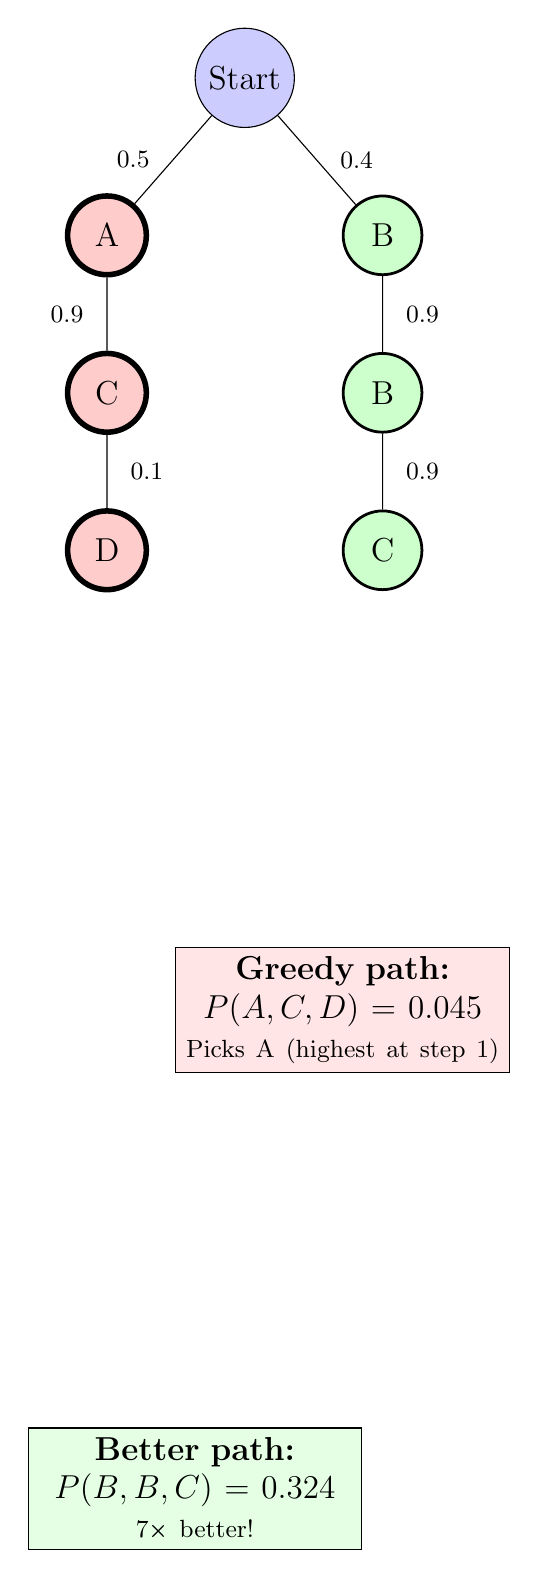
\begin{tikzpicture}[
    level distance=2cm,
    level 1/.style={sibling distance=3.5cm},
    level 2/.style={sibling distance=2cm},
    every node/.style={circle, draw, minimum size=1cm, font=\large},
    greedy/.style={fill=red!20, line width=2pt},
    better/.style={fill=green!20, line width=1pt},
    arrow/.style={->, >=stealth, very thick}
]

% Root
\node[fill=blue!20] {Start}
    child {node[greedy] {A}
        child {node[greedy] {C}
            child {node[greedy] {D}
                edge from parent node[right, rectangle, draw=none, font=\small] {0.1}
            }
            edge from parent node[left, rectangle, draw=none, font=\small] {0.9}
        }
        edge from parent node[left, rectangle, draw=none, font=\small] {0.5}
    }
    child {node[better] {B}
        child {node[better] {B}
            child {node[better] {C}
                edge from parent node[right, rectangle, draw=none, font=\small] {0.9}
            }
            edge from parent node[right, rectangle, draw=none, font=\small] {0.9}
        }
        edge from parent node[right, rectangle, draw=none, font=\small] {0.4}
    };

% Annotations
\node[rectangle, draw, fill=red!10, below=4.5cm of current bounding box.south west, xshift=4cm, text width=4cm, align=center] {
    \textbf{Greedy path:}\\
    $P(A,C,D) = 0.045$\\
    {\small Picks A (highest at step 1)}
};

\node[rectangle, draw, fill=green!10, below=4.5cm of current bounding box.south east, xshift=-4cm, text width=4cm, align=center] {
    \textbf{Better path:}\\
    $P(B,B,C) = 0.324$\\
    {\small 7× better!}
};

\end{tikzpicture}
\end{center}

The greedy choice at step 1 (token A) leads to a worse overall sequence!

\subsection{Greedy Search: Summary}

\begin{center}
\begin{tabular}{|l|c|}
\hline
\textbf{Advantage} & \textbf{Disadvantage} \\
\hline
Very fast: $O(|\mathcal{Y}| T')$ & Can miss globally optimal sequence \\
Simple to implement & No recovery from mistakes \\
Low memory & Myopic (local decisions) \\
\hline
\end{tabular}
\end{center}

\textbf{When to use}: Fast prototyping, real-time applications, well-trained models.

\section{Beam Search: A Better Heuristic}

\subsection{The Spectrum of Search Strategies}

\begin{center}
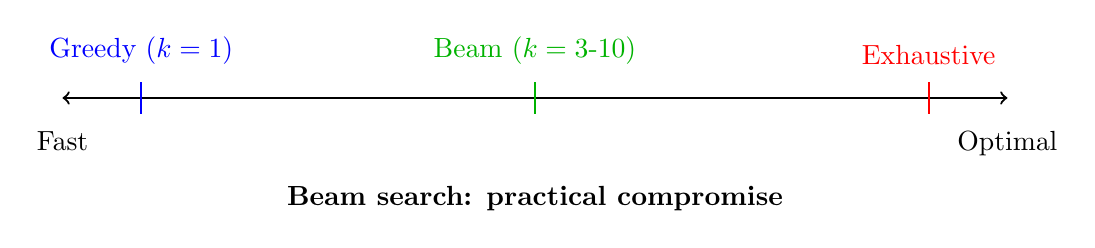
\begin{tikzpicture}
\draw[<->, thick] (0,0) -- (12,0);
\node[below] at (0,-0.3) {Fast};
\node[below] at (12,-0.3) {Optimal};

\node[above, blue] at (1,0.3) {Greedy ($k=1$)};
\draw[blue, thick] (1,-0.2) -- (1,0.2);

\node[above, green!70!black] at (6,0.3) {Beam ($k=3\text{-}10$)};
\draw[green!70!black, thick] (6,-0.2) -- (6,0.2);

\node[above, red] at (11,0.3) {Exhaustive};
\draw[red, thick] (11,-0.2) -- (11,0.2);

\node[below] at (6,-1) {\textbf{Beam search: practical compromise}};
\end{tikzpicture}
\end{center}

\subsection{Beam Search Algorithm}

\textbf{Core idea}: Maintain the top $k$ candidate sequences at each step (the ``beam width'').

\begin{tcolorbox}[colback=green!5!white, colframe=green!50!black, title=Beam Search (Section 10.8.3)]
At each timestep $t'$:
\begin{enumerate}
\item Expand each of the $k$ current hypotheses by all $|\mathcal{Y}|$ tokens
\item This creates $k \cdot |\mathcal{Y}|$ candidates
\item Keep only the top $k$ sequences by cumulative probability
\end{enumerate}

\textbf{Complexity}: $O(k \cdot |\mathcal{Y}| \cdot T')$
\end{tcolorbox}

\subsection{Visual Example: Beam Width $k=2$}

\begin{center}
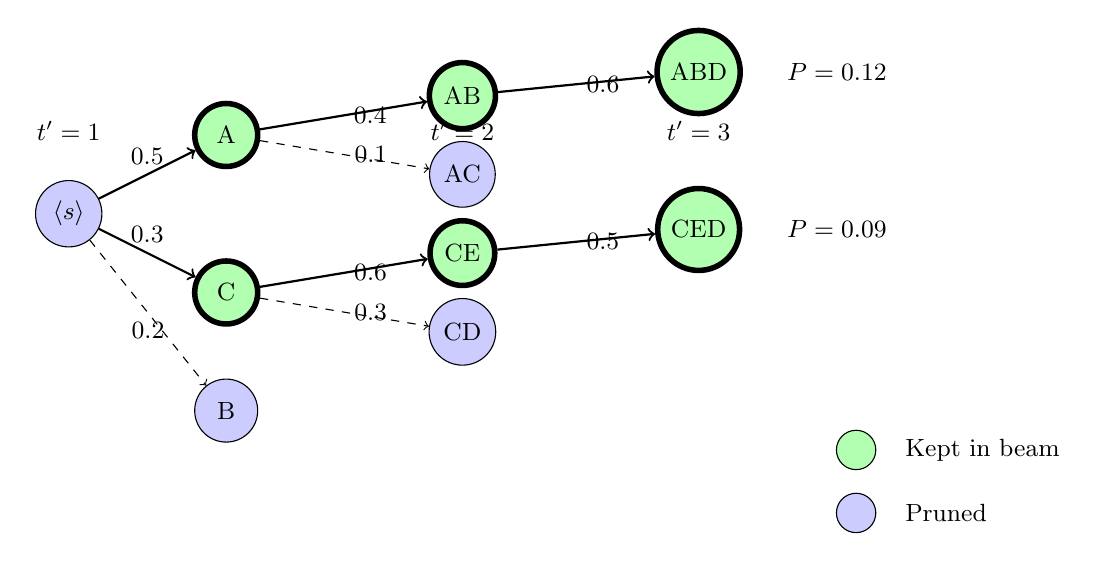
\begin{tikzpicture}[
    node distance=1.5cm,
    every node/.style={font=\small},
    candidate/.style={circle, draw, fill=blue!20, minimum size=0.8cm},
    selected/.style={circle, draw, fill=green!30, line width=2pt, minimum size=0.8cm}
]

% Time step 1
\node[candidate] (start) at (0,0) {$\langle s \rangle$};
\node[above] at (0, 0.8) {$t'=1$};

\node[selected] (a1) at (2, 1) {A};
\node[selected] (c1) at (2, -1) {C};
\node[candidate] (b1) at (2, -2.5) {B};

\draw[->, thick] (start) -- (a1) node[midway, above] {0.5};
\draw[->, thick] (start) -- (c1) node[midway, above] {0.3};
\draw[->, dashed] (start) -- (b1) node[midway, below] {0.2};

% Time step 2
\node[above] at (5, 0.8) {$t'=2$};

\node[selected] (ab2) at (5, 1.5) {AB};
\node[candidate] (ac2) at (5, 0.5) {AC};
\node[selected] (ce2) at (5, -0.5) {CE};
\node[candidate] (cd2) at (5, -1.5) {CD};

\draw[->, thick] (a1) -- (ab2) node[midway, right] {0.4};
\draw[->, dashed] (a1) -- (ac2) node[midway, right] {0.1};
\draw[->, thick] (c1) -- (ce2) node[midway, right] {0.6};
\draw[->, dashed] (c1) -- (cd2) node[midway, right] {0.3};

% Time step 3
\node[above] at (8, 0.8) {$t'=3$};

\node[selected] (abd3) at (8, 1.8) {ABD};
\node[selected] (ced3) at (8, -0.2) {CED};

\draw[->, thick] (ab2) -- (abd3) node[midway, right] {0.6};
\draw[->, thick] (ce2) -- (ced3) node[midway, right] {0.5};

% Legend
\node[right] at (9, 1.8) {$P=0.12$};
\node[right] at (9, -0.2) {$P=0.09$};

\node[draw, fill=green!30, circle, minimum size=0.5cm] at (10, -3) {};
\node[right] at (10.5, -3) {Kept in beam};
\node[draw, fill=blue!20, circle, minimum size=0.5cm] at (10, -3.8) {};
\node[right] at (10.5, -3.8) {Pruned};

\end{tikzpicture}
\end{center}

\subsection{Length Normalization}

\textbf{Problem}: Longer sequences have more probability terms to multiply, leading to smaller products. Beam search may favor shorter sequences.

\textbf{Solution}: Normalize by sequence length with penalty $\alpha$:
\[
\text{score}(\mathbf{y}) = \frac{1}{L^\alpha} \sum_{t'=1}^{L} \log P(y_{t'} \mid y_1, \ldots, y_{t'-1}, \mathbf{c})
\]

Typical values: $\alpha \in [0.6, 0.75]$

\subsection{Complexity Comparison}

\begin{center}
\begin{tabular}{|l|c|c|}
\hline
\textbf{Strategy} & \textbf{Complexity} & \textbf{Example} ($|\mathcal{Y}|=10^4, T'=10$) \\
\hline
Exhaustive & $O(|\mathcal{Y}|^{T'})$ & $10^{40}$ (intractable!) \\
Greedy ($k=1$) & $O(|\mathcal{Y}| \cdot T')$ & $10^5$ \\
Beam ($k=5$) & $O(k \cdot |\mathcal{Y}| \cdot T')$ & $5 \times 10^5$ \\
\hline
\end{tabular}
\end{center}

\subsection{Practical Guidelines}

\textbf{Choosing beam width $k$}:
\begin{itemize}
\item $k=1$: Greedy search (fastest, lowest quality)
\item $k=3$-$5$: Good default for most tasks
\item $k=10+$: Diminishing returns, much slower
\end{itemize}

\textbf{Task-specific recommendations}:
\begin{itemize}
\item Machine translation: $k=4$-$5$
\item Text summarization: $k=3$-$4$
\item Image captioning: $k=3$
\item Dialogue systems: $k=1$-$3$ (speed matters)
\end{itemize}

\begin{tcolorbox}[colback=green!5!white, colframe=green!50!black, title=Empirical Impact: Beam Search]
\textbf{Experiment}: Generate translations on test set with different decoding strategies.

\vspace{0.3cm}
\begin{center}
\begin{tabular}{|l|c|c|c|}
\hline
\textbf{Algorithm} & \textbf{Beam ($k$)} & \textbf{BLEU} & \textbf{Time (ms/sent)} \\
\hline
Greedy & 1 & 27.1 & 45 \\
Beam Search & 3 & 28.9 & 125 \\
Beam Search & 5 & 29.4 & 208 \\
\hline
\end{tabular}
\end{center}

\vspace{0.3cm}
\textbf{Key observations}:
\begin{itemize}
\item \textbf{Quality-speed tradeoff}: Beam search improves BLEU by 8.5\% ($k=5$) but increases latency 4.6×
\item \textbf{Diminishing returns}: Going from $k=3$ to $k=5$ only adds 0.5 BLEU points
\item \textbf{Sweet spot}: $k=3$ often optimal in practice
\end{itemize}
\end{tcolorbox}

\subsubsection{Qualitative Analysis: Why Beam Search Wins}

Beyond BLEU scores, examining specific translations reveals beam search's advantages:

\begin{center}
\small
\begin{tabular}{|p{4cm}|p{5cm}|p{5cm}|}
\hline
\textbf{Source (EN)} & \textbf{Greedy ($k=1$)} & \textbf{Beam ($k=5$)} \\
\hline
Two dogs are running through a field of snow. & 
Zwei Hunde rennen durch ein Feld \textbf{von Schnee}. & 
Zwei Hunde rennen durch ein \textbf{Schneefeld}. \\
\hline
The woman who is holding the camera is smiling. & 
Die Frau, die die Kamera \textbf{hält}, lächelt. & 
Die Frau, die die Kamera \textbf{in der Hand hält}, lächelt. \\
\hline
\end{tabular}
\end{center}

\textbf{Analysis}:
\begin{itemize}
\item First example: Beam search produces more idiomatic German (``Schneefeld'' vs. literal ``Feld von Schnee'')
\item Second example: Beam search captures nuance (``in der Hand hält'' = ``holding in the hand'')
\end{itemize}

These examples show beam search excels at navigating complex grammatical structures and making nuanced lexical choices where greedy search's myopia causes failures.

\begin{lstlisting}[language=Python, caption=Beam Search Implementation Sketch]
def beam_search(model, encoder_output, k=3, max_len=50):
    # Initialize with k beams
    beams = [(sequence=[BOS_TOKEN], score=0.0)]
    
    for t in range(max_len):
        candidates = []
        
        # Expand each beam
        for seq, score in beams:
            if seq[-1] == EOS_TOKEN:
                candidates.append((seq, score))
                continue
            
            logits = model.decoder(seq, encoder_output)
            probs = F.softmax(logits[-1])
            
            # Get top-k tokens for this beam
            top_k_probs, top_k_tokens = probs.topk(k)
            
            for prob, token in zip(top_k_probs, top_k_tokens):
                new_seq = seq + [token]
                new_score = score + log(prob)
                candidates.append((new_seq, new_score))
        
        # Keep top-k candidates (with length normalization)
        candidates.sort(key=lambda x: x[1] / len(x[0])**alpha, 
                        reverse=True)
        beams = candidates[:k]
    
    return beams[0][0]  # Return best sequence
\end{lstlisting}

\section{Summary \& Looking Ahead}

\subsection{Consolidated Performance Gains}

The following table synthesizes all empirical results, showing cumulative improvements over baseline:

\begin{center}
\small
\begin{tabular}{|l|l|c|c|}
\hline
\textbf{Stage/Technique} & \textbf{Metric} & \textbf{Result} & \textbf{Improvement} \\
\hline
\multirow{2}{*}{Baseline Model} & Training time/epoch & 18.5 min & — \\
 & BLEU score & 19.8 & — \\
\hline
+ Teacher Forcing & Training time/epoch & 2.1 min & \textbf{88.6\% faster} \\
\hline
+ Scheduled Sampling & BLEU score & 27.1 & \textbf{+36.9\%} \\
\hline
+ Sequence Bucketing & Throughput (sent/sec) & 31 & \textbf{+72\%} \\
\hline
+ Beam Search ($k=5$) & BLEU score & 29.4 & \textbf{+48.5\%} \\
\hline
\end{tabular}
\end{center}

\vspace{0.5cm}

\textbf{The Holistic View}: Different techniques address distinct bottlenecks:
\begin{itemize}
\item \textbf{Training speed}: Teacher forcing (8.8× speedup)
\item \textbf{Generalization}: Scheduled sampling (+6.7\% BLEU)
\item \textbf{Inference throughput}: Sequence bucketing (72\% faster)
\item \textbf{Output quality}: Beam search (+8.5\% BLEU)
\end{itemize}

\subsection{Key Takeaways}

\textbf{Training Techniques}:
\begin{itemize}
\item \textbf{Teacher forcing} accelerates training by using ground-truth inputs
\begin{itemize}
\item Provides stable gradients and clean learning signal
\item Can reduce training time by an order of magnitude
\item Empirical gain: 88.6\% reduction in time per epoch
\end{itemize}
\item \textbf{Scheduled sampling} mitigates exposure bias by gradually transitioning to model predictions
\begin{itemize}
\item Use curriculum learning: start with $\epsilon=1.0$ (full teacher forcing), decay to $\epsilon \approx 0.0$
\item \textit{Never} start with $\epsilon=0$ (always sampling)—model cannot learn
\item Flip coin per token, not per sequence
\item Choose decay schedule based on task (inverse sigmoid often works well)
\item Empirical gain: +6.7\% BLEU score improvement
\end{itemize}
\item \textbf{Masking} ensures padded tokens don't corrupt gradients or loss
\end{itemize}

\textbf{Inference Strategies}:
\begin{itemize}
\item \textbf{Sequence bucketing} dramatically improves throughput by minimizing padding waste
\begin{itemize}
\item Empirical gain: 72\% increase in throughput, 82\% reduction in padding
\item Hardware-aware optimization—no model changes needed
\end{itemize}
\item \textbf{Greedy search} is fast but myopic—can miss better sequences
\item \textbf{Beam search} balances quality and speed, standard in production systems
\begin{itemize}
\item Empirical gain: +8.5\% BLEU, but 4.6× slower than greedy
\item Typical sweet spot: $k=3$-$5$
\end{itemize}
\end{itemize}

\subsection{Connection to Curriculum Learning}

Scheduled sampling is an instance of \textbf{curriculum learning} (Bengio et al., 2009): organizing training examples from easy to hard.

\textbf{The curriculum}:
\begin{enumerate}
\item \textbf{Easy task}: Predict next token given ground-truth context (teacher forcing)
\begin{itemize}
\item Model always sees perfect history
\item Stable gradients, fast initial learning
\end{itemize}
\item \textbf{Medium task}: Mix of ground-truth and model predictions ($0 < \epsilon < 1$)
\begin{itemize}
\item Model begins to see its own mistakes
\item Learns to recover from errors
\end{itemize}
\item \textbf{Hard task}: Predict given model's own predictions ($\epsilon \approx 0$)
\begin{itemize}
\item Matches inference conditions
\item Model robust to accumulated errors
\end{itemize}
\end{enumerate}

\textbf{Why does this work?} Early in training, the model produces random outputs. Feeding random tokens back would prevent learning. By gradually exposing the model to its own (improving) predictions, we enable stable learning while building robustness.

\subsection{The Road to Transformers}

These techniques aren't just for RNNs—they're fundamental to modern deep learning:

\begin{tcolorbox}[colback=yellow!5!white, colframe=orange!50!black, title=Foundational Concepts]
\begin{itemize}
\item \textbf{Teacher forcing}: Used in autoregressive Transformers (GPT, etc.)
\item \textbf{Masking}: Critical for attention mechanisms (padding + causal masks)
\item \textbf{Bucketing}: Essential for efficient Transformer inference
\item \textbf{Beam search}: Standard decoding for neural machine translation (with Transformers!)
\end{itemize}

\textbf{Next lecture}: We'll see how Transformers achieve the parallelization potential hinted at by teacher forcing, and how attention mechanisms eliminate the need for recurrence entirely.
\end{tcolorbox}

\subsection{Practical Advice}

\textbf{For your projects}:
\begin{enumerate}
\item \textbf{Establish baselines}: Always measure performance before optimizing
\item \textbf{Always use teacher forcing} during training (at least initially)
\item \textbf{Implement proper masking} for variable-length sequences
\item \textbf{Use sequence bucketing} for batch inference in production
\item \textbf{Start with greedy decoding}, upgrade to beam search if quality matters
\item \textbf{Monitor the train-test gap}—it may indicate exposure bias
\item \textbf{Measure empirically}: Don't assume—benchmark every optimization
\end{enumerate}

\begin{tcolorbox}[colback=orange!5!white, colframe=orange!50!black, title=The Empirical Mindset]
The principles demonstrated here extend beyond RNNs:
\begin{itemize}
\item \textbf{Establish baselines} before claiming improvements
\item \textbf{Understand trade-offs} (speed vs. quality, training vs. inference)
\item \textbf{Optimize data pipelines} alongside model architecture
\item \textbf{Refine search algorithms} for better generation
\item \textbf{Measure everything}: Training time, inference latency, memory usage, and task metrics
\end{itemize}

These habits are fundamental to effective application of \textit{all} deep learning models, not just RNNs.
\end{tcolorbox}

\subsection{The Triple Constraint in Practice}

Returning to our opening framework, we've seen how to navigate the triple constraint:

\begin{center}
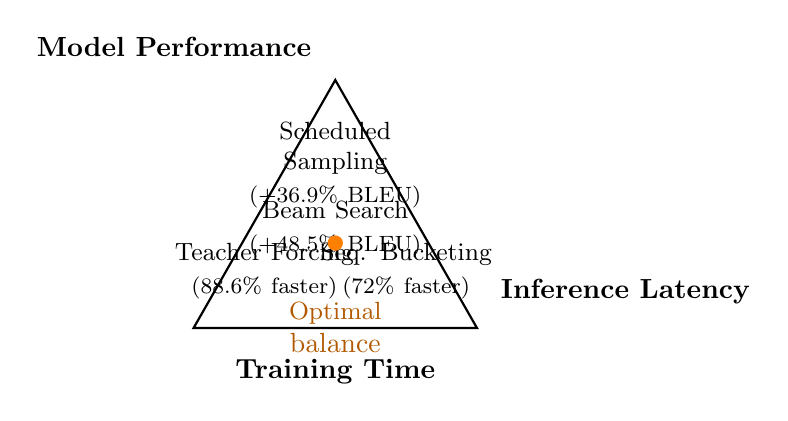
\begin{tikzpicture}[scale=0.9]
% Triangle
\draw[thick] (0,0) -- (4,0) -- (2,3.5) -- cycle;

% Labels at vertices
\node[below] at (2, -0.3) {\textbf{Training Time}};
\node[above right] at (4.2, 0.2) {\textbf{Inference Latency}};
\node[above left] at (1.8, 3.7) {\textbf{Model Performance}};

% Solutions in each region
\node[align=center, text width=2.5cm] at (1, 0.8) {\small Teacher Forcing\\ \footnotesize (88.6\% faster)};
\node[align=center, text width=2.5cm] at (3, 0.8) {\small Seq. Bucketing\\ \footnotesize (72\% faster)};
\node[align=center, text width=2.5cm] at (2, 2.3) {\small Scheduled Sampling\\ \footnotesize (+36.9\% BLEU)};
\node[align=center, text width=2.5cm] at (2, 1.4) {\small Beam Search\\ \footnotesize (+48.5\% BLEU)};

% Center
\filldraw[orange] (2, 1.2) circle (0.1);
\node[below, orange!70!black, align = center] at (2, 0.5) {\small Optimal\\ balance};
\end{tikzpicture}
\end{center}

No single technique solves all problems. Success requires understanding which bottleneck matters most for your application and applying the appropriate optimization.

\end{document}